%%%%%%%%%%%%%%%%%%%%%%%%%%%%%%%%%%%%%%%%%%%%%%%%%%%%%%%%%%%%%%%%%%%%%%%%%%
%%%%%                        Intro Générale                         %%%%%%
%%%%%%%%%%%%%%%%%%%%%%%%%%%%%%%%%%%%%%%%%%%%%%%%%%%%%%%%%%%%%%%%%%%%%%%%%%
\phantomsection 
\addcontentsline{toc}{chapter}{Preamble}
\addtocontents{toc}{\protect\addvspace{10pt}}

\vspace*{-1cm}
\begin{flushright}
\section*{\fontsize{20pt}{20pt}\selectfont\textnormal{Preamble}}
\end{flushright}
\vspace{2cm}

\lhead[\fancyplain{}{Preamble}]
      {\fancyplain{}{}}
\chead[\fancyplain{}{}]
      {\fancyplain{}{}}
\rhead[\fancyplain{}{}]
      {\fancyplain{}{Preamble}}
\lfoot[\fancyplain{}{}]%
      {\fancyplain{}{}}
\cfoot[\fancyplain{}{\thepage}]
      {\fancyplain{}{\thepage}}
\rfoot[\fancyplain{}{}]%
     {\fancyplain{}{\scriptsize}}
     

%%%%%%%%%%%%%%%%%%%%%%%%%%%%%%%%%%%%%%%%%%%%%%%%%%%%%%%%%%%%%%%%%%%%%%%%%%
%%%%%                      Start part here                          %%%%%%
%%%%%%%%%%%%%%%%%%%%%%%%%%%%%%%%%%%%%%%%%%%%%%%%%%%%%%%%%%%%%%%%%%%%%%%%%%

\section*{Working Environment}

This doctoral thesis was undertaken from December 2nd, 2019 to November 30th, 2022, at the LJK (Laboratoire Jean Kuntzmann for Applied Mathematics and Informatics) in Grenoble, France. It was funded by the French National Center for Scientific Research (CNRS), 
through the program "thèses transverses" of the Mission pour les Initiatives
Transverses et Interdisciplinaires (MITI).
% as the result of a collaboration between the PPrime Institute (UPR3346, Poitiers, France), the French Cycling Federation (FFC), and the INSEP (French National Institute of Sport, Expertise and Performance), through the CREPS of Poitiers (Center for Sport Resource, Expertise, and Performance) and TSF Voiron (Springboard for Sports Training). 
It was later incorporated into the PerfAnalytics project, which aims to boost French sports performance for the 2024 Olympic Games in Paris, with a particular focus on video analysis.


\section*{Context}

Currently, the analysis of sports performance is still mostly carried out by subjective visual examination. More objective approaches exist, but they are usually complex and cumbersome to implement, or inappropriate for in-situ analysis. Hence, coaches rarely find them practical for daily use. In order to address this issue, other methods are being developed, among which many focus on video analysis. One of the long-term objectives in this area is to be able to quantify the full-body kinematics and dynamics of athletes in context, without interfering with their training or competition, in a clear and timely way, so as for coaches to be able to give them a fast, accurate, objective, and comprehensive feedback on their technique and tactics. New algorithms are regularly released estimating 3D pose from one single camera, but they are more adapted for character animation in the entertainment industry than for precise motion analysis. In order to meet sports accuracy requirement, it appeared to us that the most appropriate method would take advantage of the video streams provided by a network of calibrated cameras. Each stream would be processed by some preexisting 2D keypoint detection deep-learning models. These coordinates would then be triangulated, and finally be constrained to a biomechanically consistent full-body skeletal model. 

The original goal of this thesis shifted along the program, as it was initially intended mostly for bicycle motocross (BMX) racing performance analysis. BMX racing presented a lot of challenges which needed to be first addressed, such as the large size of the field of view, the direct sunlight, the swiftness of the movements, the occlusions of the pilot by the bike, and the lack of facilities for setting up the capture hardware. As a consequence, we first started with studying walking, running, and cycling tasks indoors, with a virtual and controlled environment map simulating an outdoor scene. We then studied boxing key performance indicators (KPIs) with lightweight consumer-grade hardware, and finally moved outdoors to investigate BMX racing.


\begin{textblock*}{10cm}(5cm,30.7cm) % {block width} (coords left,top) 
      \begin{turn}{0}  
            \scriptsize \emojiegg
            \tiny 1. Merci Maman ! 
            \scriptsize \emojimedal
      \end{turn}
\end{textblock*}


\newpage
\section*{Content}

The thesis is organized as follows:
\vskip 0.4cm
\noindent\autoref{ch:1}: \emph{State of the art of sports motion analysis}. \newline
Motion capture is traditionally performed with marker-based systems. However, these solutions are generally incompatible with on-field sports analysis, as they involve marker placement on the skin, and a heavy setup. Consequently, markerless approaches are being investigated. 
\vskip 0.4cm
\noindent\autoref{ch:2}: \emph{From computer vision to biomechanics}. \newline
One of the most promising prospects for sports motion analysis lies at the intersection of machine learning for 2D pose estimation, computer vision for 3D reconstruction from multiple video sources, and biomechanics for constraining coordinates to an anatomically consistent model. 
\vskip 0.4cm
\noindent\autoref{ch:3}: \emph{A practical implementation}. \newline
Sports scientists would benefit from having access to a user-friendly integrated workflow for on-field analysis. Hence, Pose2Sim, an open-source Python package striving to answer these needs, has been proposed and released. 2D keypoint coordinates obtained with OpenPose or DeepLabCut are robustly triangulated, and serve as input for a full-body OpenSim inverse kinematics procedure \cite{Pagnon2022b}.
\vskip 0.4cm
\noindent\autoref{ch:4}: \emph{Robustness assessment}. \newline
Pose2Sim robustness has been evaluated for people entering and exiting the field of view, degraded image quality, calibration errors, and low number of cameras \cite{Pagnon2021}. 
\vskip 0.4cm
\noindent\autoref{ch:5}: \emph{Accuracy assessment}. \newline
Its accuracy has also been assessed, and deemed sufficient for walking, running, and cycling analysis \cite{Pagnon2022a}. 
\vskip 0.4cm
\noindent\autoref{ch:6}: \emph{Using consumer-grade hardware}. \newline
In the context of competition, research-grade hardware is not always workable as it is cumbersome and complex to set up. We tested the use of GoPro cameras and proposed a method for calibrating and synchronizing them. The workflow was applied to shadow-boxing, which involves fast, three-dimensional, full-body movements. The measure of Key Performance Indicators (KPIs) was concurrently validated with a marker-based protocol, and demonstrated to be remarkably accurate \cite{Pagnon2022c}.
\vskip 0.4cm
\noindent\autoref{ch:7}: \emph{Capturing equipment along with the athlete}. \newline
Numerous sports disciplines are practiced with dedicated equipment, whose motion is important to retrieve. However, this equipment can form a closed loop with the athlete, which makes the task mathematically challenging to resolve. We analyzed a BMX race starting sequence using OpenPose for human pose estimation, a custom trained DeepLabCut model for bike detection, and a custom OpenSim \{pilot+bike\} model for kinematic analysis. Expected KPI patterns were successfully measured, but results were inconclusive when constraints were added between the pilot and their equipment \cite{Pagnon2022e}.


\begin{textblock*}{10cm}(15cm,22.5cm) % {block width} (coords left,top) 
      \begin{turn}{0}  
            \scriptsize \emojiegg
            \tiny 2. Thank you, Mikaela! 
            \scriptsize \emojibell
      \end{turn}
\end{textblock*}


% OpenSim model constraining handles to hands, and pedals to feet. The field was too large, and the image quality too low to obtain good results. However, we previously captured marker data of a similar scene. Keeping only markers similar to those detected by OpenPose and DeepLabCut, we were able to run the analysis. As a consequence, we hypothesize that assuming a sufficiently good image quality, it would be possible to provide joint \{bike+pilot\} kinematics to coaches. 

% \begin{figure}[hbtp]
% 	\centering
%             \def\svgwidth{1\columnwidth}
%             \fontsize{10pt}{10pt}\selectfont
%             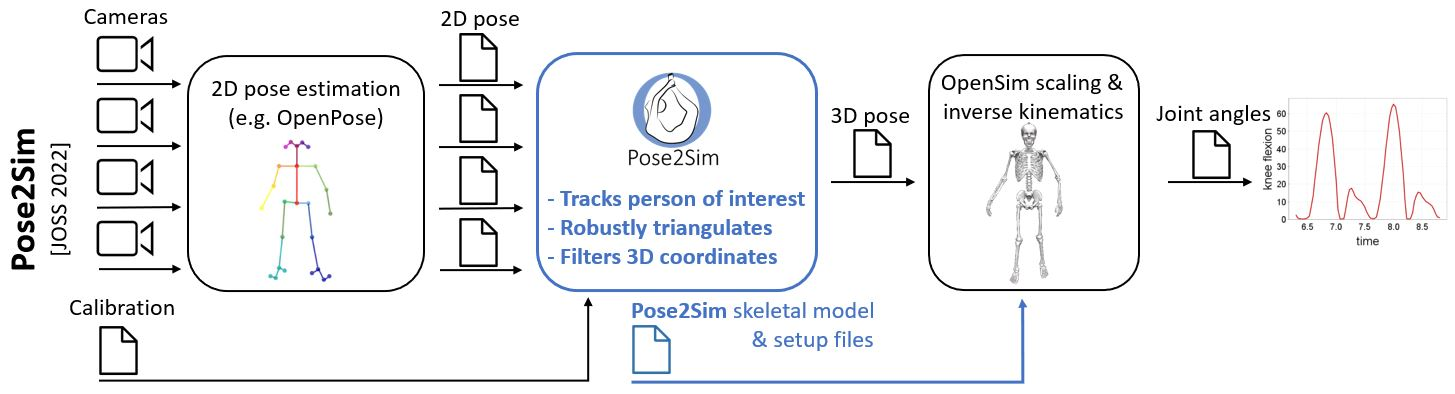
\includegraphics[width=\linewidth]{"../Intro/Figures/Fig_VisAbstract1.JPG"}
%             \caption{Visual abstract for the Pose2Sim workflow (\autoref{ch:3}) \cite{Pagnon2022b}.}
%             \label{fig_visabstract1_1}
% \end{figure}

% \begin{figure}[!htp]
% 	\centering
% 	\begin{subfigure}[b]{1\textwidth}
%             \centering
%             \def\svgwidth{1\columnwidth}
%             \fontsize{10pt}{10pt}\selectfont
%             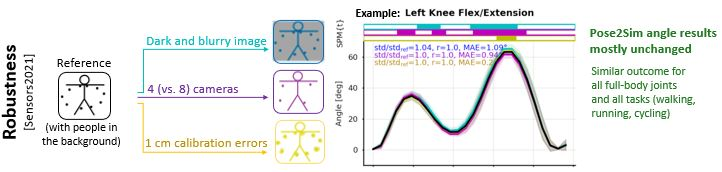
\includegraphics[width=\linewidth]{"../Intro/Figures/Fig_VisAbstract2.JPG"}
%             \caption{Visual abstract for Pose2Sim robustness assessment (\autoref{ch:4}) \cite{Pagnon2021}.}
%             \label{fig_visabstract2_1}
% 	\end{subfigure}
% 	\vskip 0.8cm
%       \begin{subfigure}[b]{1\textwidth}
%             \centering
%             \def\svgwidth{1\columnwidth}
%             \fontsize{10pt}{10pt}\selectfont
%             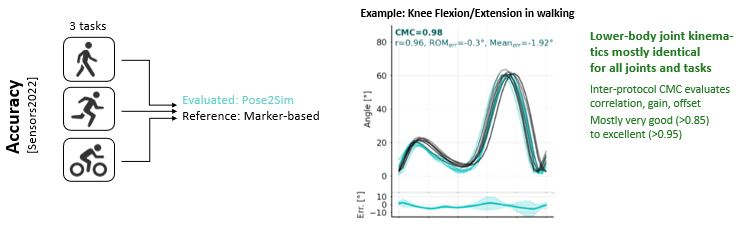
\includegraphics[width=\linewidth]{"../Intro/Figures/Fig_VisAbstract3.JPG"}
%             \caption{Visual abstract for Pose2Sim accuracy assessment (\autoref{ch:5}) \cite{Pagnon2022a}.}
%             \label{fig_visabstract3_1}
% 	\end{subfigure}
%       \vskip 0.8cm
% 	\begin{subfigure}[b]{1\textwidth}
%             \centering
%             \captionsetup{justification=centering}
%             \def\svgwidth{1\columnwidth}
%             \fontsize{10pt}{10pt}\selectfont
%             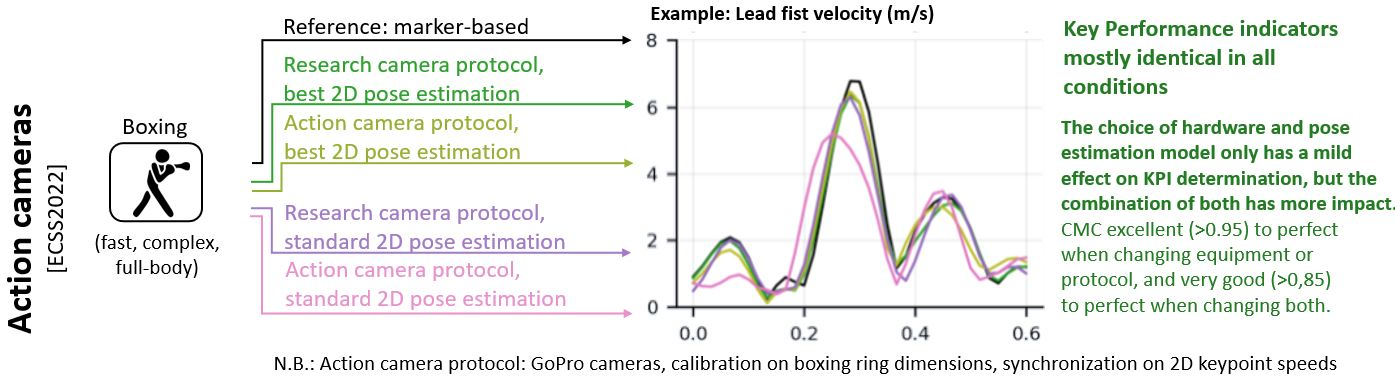
\includegraphics[width=\linewidth]{"../Intro/Figures/Fig_VisAbstract4.JPG"}
%             \caption{Visual abstract for the assessment of KPIs in boxing with Pose2Sim (\autoref{ch:6}) \cite{Pagnon2022c}. \\Research camera protocol: Qualisys cameras, calibration with markers, hardware synchronization. \\Action camera protocol: GoPro cameras, calibration on boxing ring dimensions, synchronization on 2D keypoint speeds.}
%             \label{fig_visabstract4_1}
% 	\end{subfigure}
%       \vskip 0.8cm
%       \begin{subfigure}[b]{1\textwidth}
%             \centering
%             \def\svgwidth{1\columnwidth}
%             \fontsize{10pt}{10pt}\selectfont
%             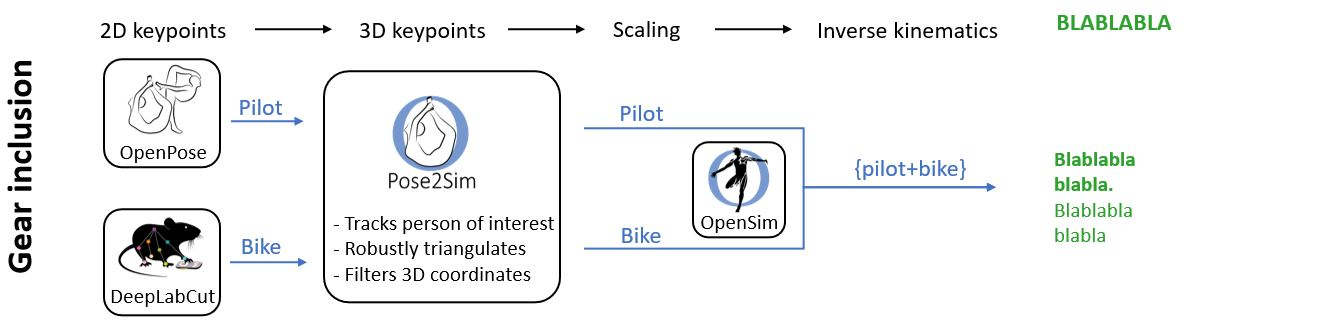
\includegraphics[width=\linewidth]{"../Intro/Figures/Fig_VisAbstract5.JPG"}
%             \caption{Visual abstract for joint analysis of the athlete with OpenPose, and their equipment with DeepLabCut (\autoref{ch:7}).}
%             \label{fig_visabstract5_1}
% 	\end{subfigure}
% 	\vskip 0.8cm
% 	\caption{Visual abstracts for chapters 4 to 7.}
% 	\label{fig_visabstract}
% \end{figure}


\newpage
\section*{Scientific contributions}

This work led to the publication of a few scientific contributions as a first author: three peer-reviewed articles, two conference talks as a first author and one as a secondary author, and the release of an open-source package.
% , and a Blender add-on integrated the published package, for 3D character animation. 
Another peer-reviewed article has been published as a first author during this period, although it was not related to the program.

\noindent\cite{Pagnon2021}: David Pagnon, Mathieu Domalain and Lionel Reveret. \textit{Pose2Sim: An
End-to-End Workflow for 3D Markerless Sports Kinematics—Part 1:
Robustness.} Sensors, vol. 21, no. 19, 2021.

\noindent\cite{Pagnon2022a}: David Pagnon, Mathieu Domalain and Lionel Reveret. \textit{Pose2Sim: An
End-to-End Workflow for 3D Markerless Sports Kinematics—Part 2:
Accuracy.} Sensors, vol. 22, no. 7, 2022.

\noindent\cite{Pagnon2022b}: David Pagnon, Mathieu Domalain and Lionel Reveret. \textit{Pose2Sim:
An open-source Python package for multiview markerless kinematics.}
Journal of Open Source Software, vol. 7, no. 77, page 4362, 2022.

\noindent\cite{Pagnon2022c}: 
David Pagnon, Mathieu Domalain, Thomas Robert, Bhrigu-Kumar Lahkar, Issa Moussa, Guillaume Saulière, Thibault Goyallon and Lionel Reveret. \textit{A 3D markerless protocol with action cameras – Key performance indicators in boxing.} In 2022 Congress of the European College of Sport Science (ECSS), Sevilla (Spain), 2022. Poster.

\noindent\cite{Lahkar2022a}: 
Bhrigu-Kumar Lahkar, Thibault Goyallon, Anaïs Chaumeil, David Pagnon, Issa Moussa, Andreas Muller, Mathieu Domalain, Lionel Reveret, Raphael Dumas, Thomas Robert. \textit{Assessment of a markerless motion capture system for upper extremity joint kinematics during boxing.} In 17th International Symposium on 3-D Analysis of Human Movement, Tokyo (Japan), 2022. Oral.

% \noindent\cite{Barreto2022}: 
% Carlos Barreto, CEB Studio. \textit{Mocap MPP2SOS} [Blender add-on], Blender Marker, 2022. \url{https://blendermarket.com/products/mocap-mpp2soss}.

\noindent\cite{Pagnon2022e}: 
David Pagnon. \textit{Markerless kinematic analysis of a BMX pilot with their equipment}. In 2022 Rencontres scientifiques de la haute performance en cyclisme, Paris (France). Oral.

\noindent\cite{Pagnon2022d}: 
David Pagnon, Germain Faity, Galo Maldonado, Yann Daout, Sidney Grosprêtre. \textit{What Makes Parkour Unique? A Narrative Review Across Miscellaneous Academic Fields.} Sports Medicine, vol. 52, page 1029, 2022.
